% Author: Johannes Borgqvist
% Date: 2020-04-20
% Description: 
% Draws a system with an activator inhhibitor system with a positive 
% deedback loop
%------------------------------------------------------------------------
%The document
%------------------------------------------------------------------------
\documentclass[tikz, border=10pt]{standalone}
%------------------------------------------------------------------------
% Usepackages
%------------------------------------------------------------------------
\usepackage{verbatim}
%------------------------------------------------------------------------
% Libraries in tikz
%------------------------------------------------------------------------
\usetikzlibrary{arrows}
\usetikzlibrary{positioning}
%------------------------------------------------------------------------
% Define some nice colors
%------------------------------------------------------------------------
\definecolor{myBlue}{RGB}{85,173,228}
%------------------------------------------------------------------------
% Setting up the document
%------------------------------------------------------------------------
\begin{document}
%------------------------------------------------------------------------
% Setting up the plot
%------------------------------------------------------------------------
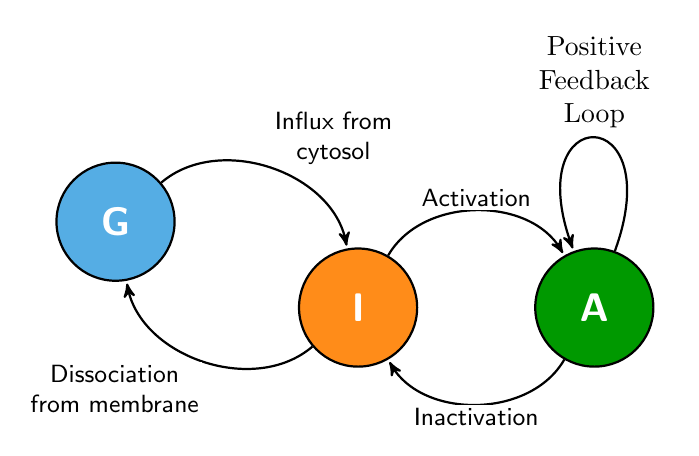
\begin{tikzpicture}[->,>=stealth',shorten >=1pt,auto,node distance=1.5cm,
  thick,main node/.style={circle,fill=green!60!black,draw,
  font=\sffamily\Large\bfseries,minimum size=15mm},second node/.style={circle,fill=orange!90,draw,
  font=\sffamily\Large\bfseries,minimum size=15mm},third node/.style={circle,fill=myBlue,draw,
  font=\sffamily\Large\bfseries,minimum size=15mm}]
%------------------------------------------------------------------------
% The Activator and the inhibitor
%------------------------------------------------------------------------
\node[second node] (A) {\color{white}I};
\node (B) [right of=A]{};
\node (C) [above right=0.65cm and 0.9cm of A]{};
\node[third node] (D) [above left=0.01cm and 2cm of A]{\color{white}G};
 \node[main node] (I) [right of=B] {\color{white}A};
%------------------------------------------------------------------------
% The reactions
%------------------------------------------------------------------------
  \path[every node/.style={font=\sffamily\small,
  		fill=white,inner sep=1pt}]{
(A) edge  [bend left=60] node{Activation} (I)% Activation reaction
(I) edge  [bend left=60] node{Inactivation} (A)% Inactivation reaction
(D) edge  [bend left=60,align=center] node{Influx from\\cytosol} (A)% Activation reaction
(A) edge  [bend left=60,align=center] node{Dissociation\\from membrane} (D)% Inactivation reaction
};
% The positive feedback loop
 \draw[thick,->](I) edge[out=70,in=110,looseness=10] node[above,align=center]{Positive\\Feedback\\Loop} (I);

\end{tikzpicture}
\end{document}
